\graphicspath{{figures/Design/IPController/}}
\chapter{Design of the Inverted Pendulum Controller}\label{sec:IPController}
The goal of the controller is to balance the stick in an upright position. 
The system is inherently unstable as is evident by the pole in the right half plane of the pole-zero plot as seen on \autoref{fig:pzip}.

\begin{figure}[htbp]
\centering
\missingfigure{}
\caption{Pole-zero plot for the inverted pendulums transfer function.}
\label{fig:pzip}
\end{figure}
\todo[inline,author=Jacob]{Missing constants from motor test to do plot.}

There's a plethora of different options for the controller to use, the simplest being a proportional controller. A simple way to check whether the proportional controller is feasible is by examining the root locus of the transfer function in figure \autoref{fig:locusIP}. The pole in the right half plane moving towards infinity is caused by the transfer function being negative and can be fixed with a negative gain as shown on figure \autoref{fig:locusNegative}.

\begin{figure}[htbp]
\centering
\missingfigure{}
\caption{Root locus of the inverted pendulums transfer function.}
\label{fig:locusIP}
\end{figure}

\begin{figure}[htbp]
\centering
\missingfigure{}
\caption{Root locus of the inverted pendulums transfer function with a negative gain.}
\label{fig:locusNegative}
\end{figure}

The proportional controller isn't feasible as the pole in the right half plane never enters the stable region even with a negative gain.

There are two options to bring the unstable pole into the stable region: The zero in 0 can be cancelled allowing the unstable pole to cross the imaginary axis along the real axis or another pole can be added in the right half plane forcing both off the real axis with a high enough gain. The second method requires a zero in the left half plane to pull the poles towards the stable region.

Cancelling zeros in 0 by adding poles can be dangerous as the steady state error will no longer be zero which is critical for a stable inverted pendulum. The system is difficult to control as the transfer function was derived with an attempt to control the angle of the stick. This is only really possible in the special case where the reference is exactly 0 at all times. The system can instead be redefined as trying to control the position of a point on the stick in relation to the vertical axis. By controlling the position instead of the angle would mean the system would still have to balance the stick but not be forced to use a reference of 0 at all times. This could make the system easier to control.

\section{Redefining the inverted pendulums output and reference point}

The inverted pendulum model will be redefined so the output is the distance a point on the stick to the vertical axis instead of the angle of the stick. The point, $\alpha$, and the distance to the vertical axis, $x_\alpha$, are seen on \autoref{fig:modelDist}.

\begin{figure}[htbp]
\centering
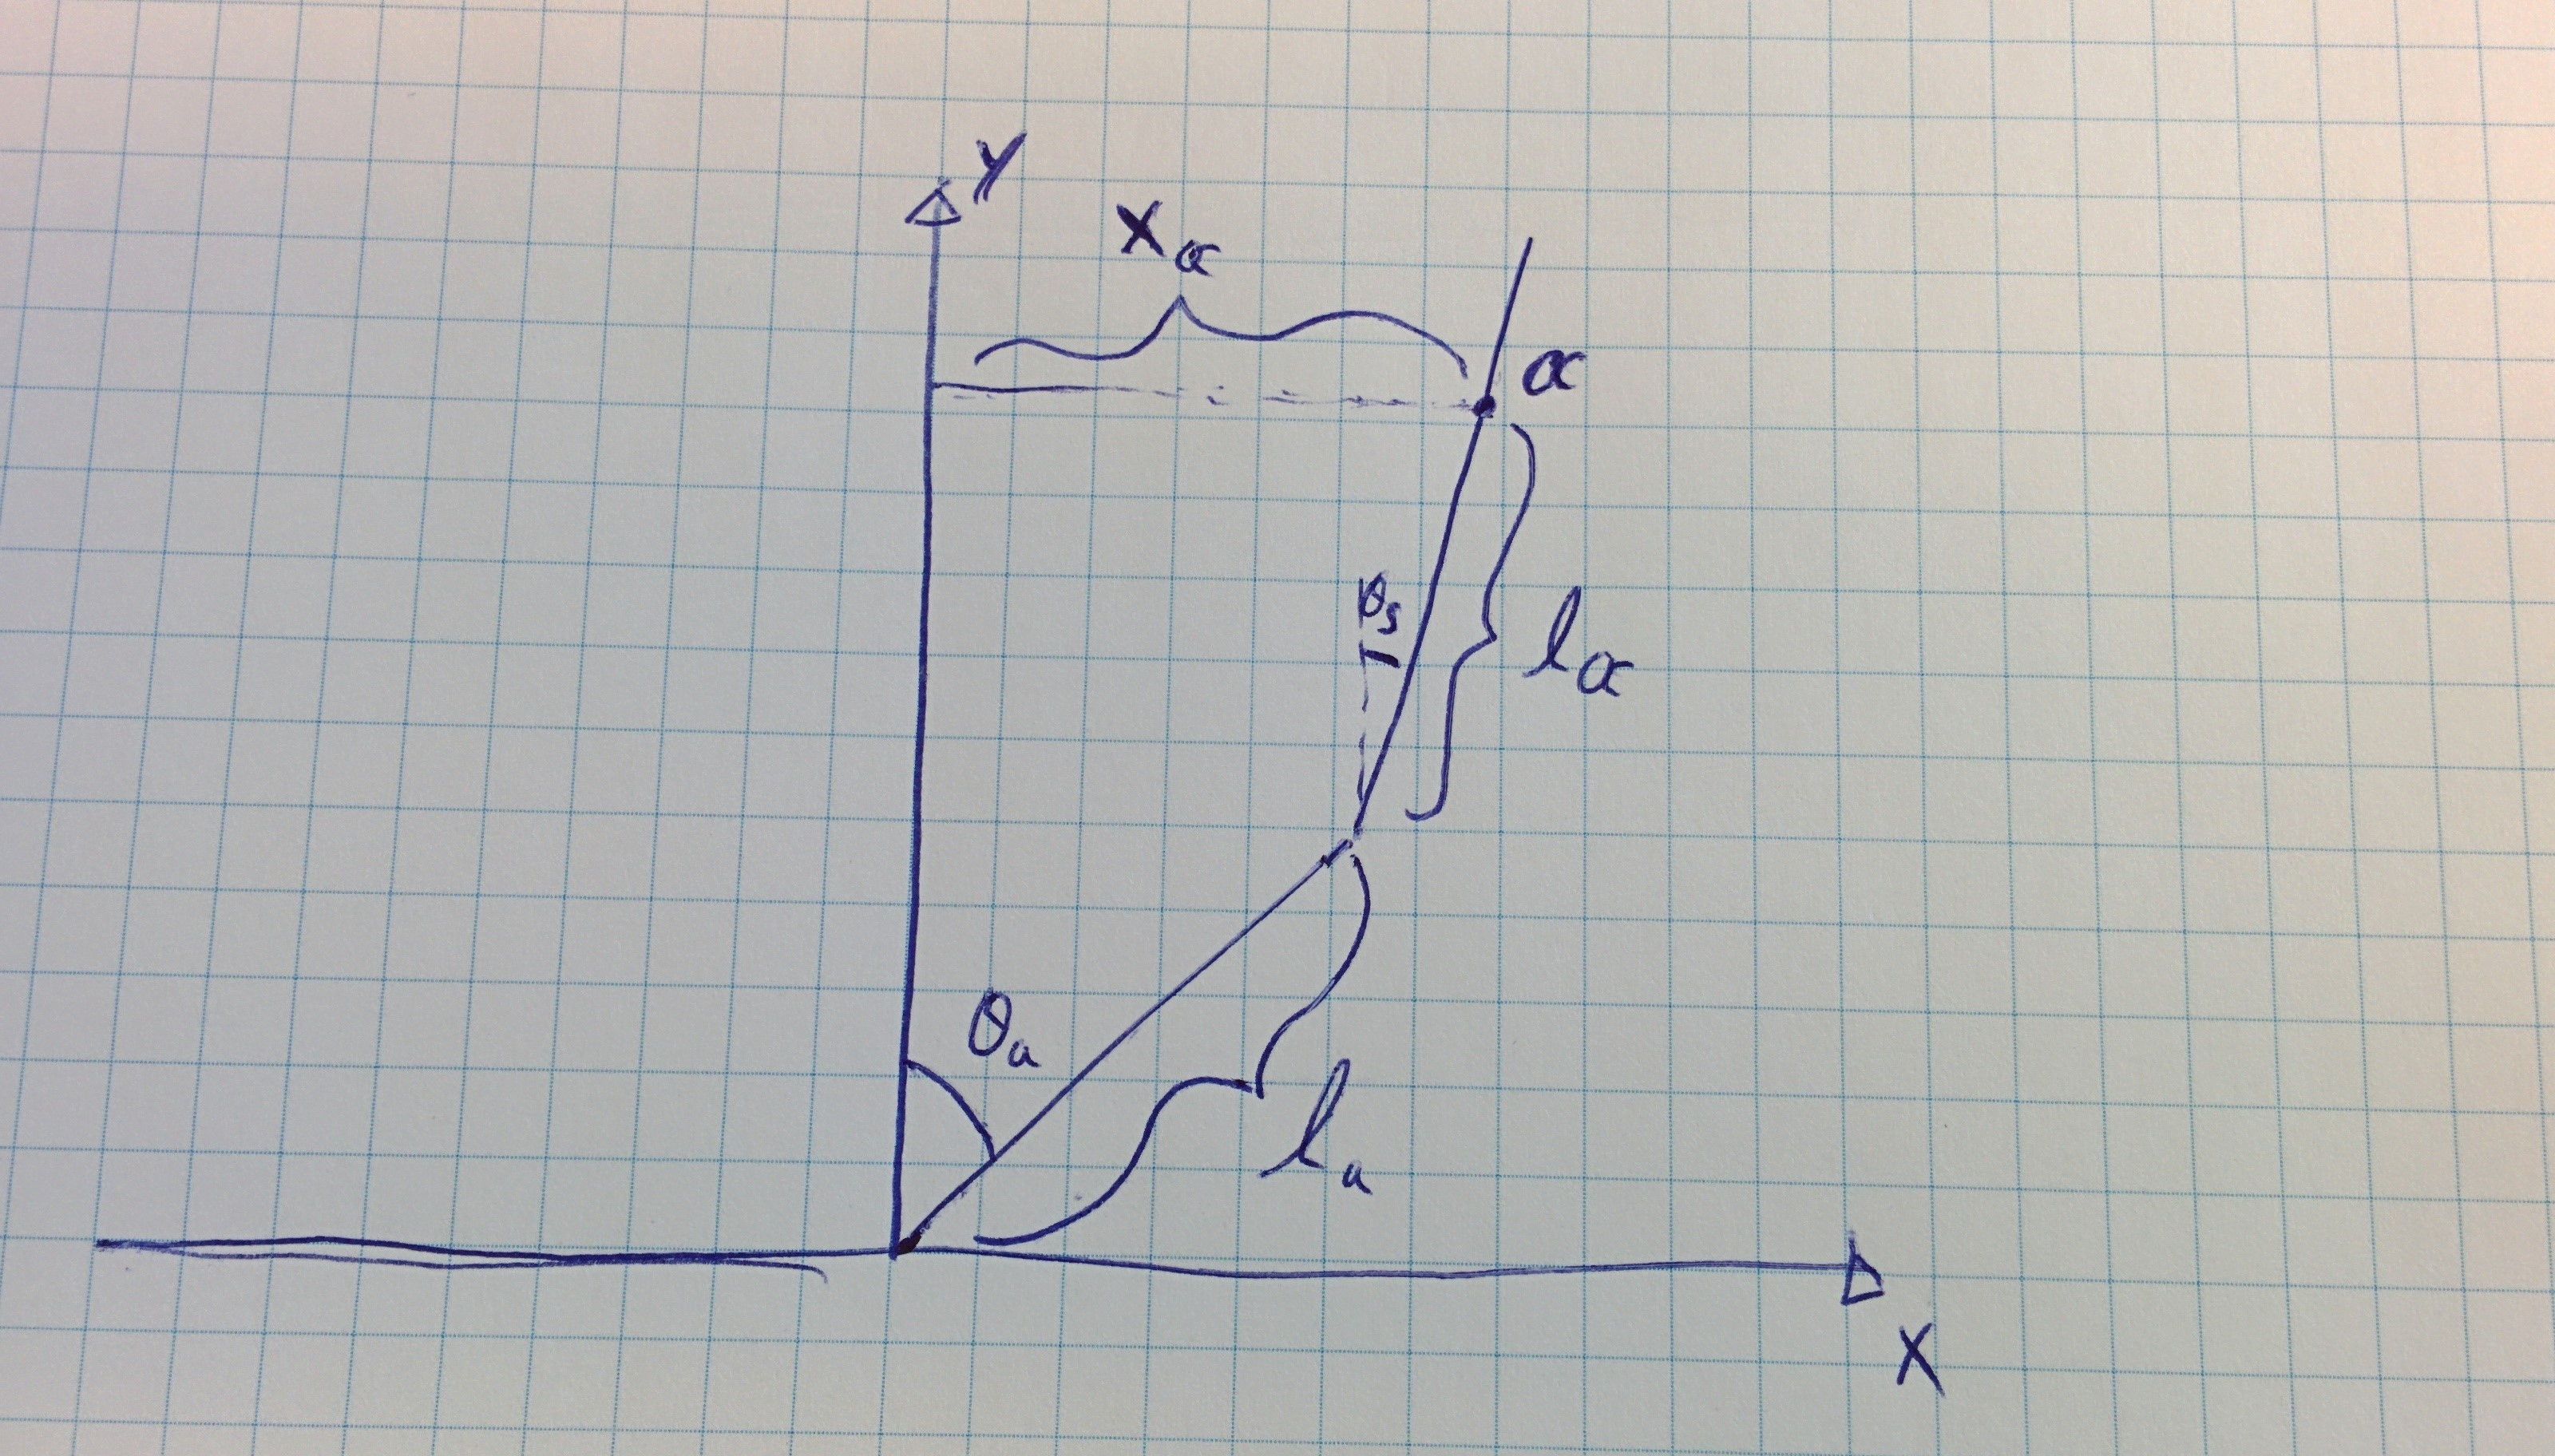
\includegraphics[width=0.7\textwidth]{ModelDist}
\caption{Diagram of the distance that will be controlled instead of the angle of the stick.}
\label{fig:modelDist}
\end{figure}

The distance to the point, $\alpha$, can be described by \autoref{eq:xa}.
\begin{flalign}\label{eq:xa}
& x_\alpha(t) = l_a\sin(\theta_a(t))+l_\alpha\sin(\theta_s(t))
\end{flalign}
This is not a linear equation and needs to be linearized in order to Laplace transform it. This is done with a 1st order Taylor approximation around the equilibrium where $\theta_a=\theta_s=0$ in \autoref{eq:xaTaylor}
\begin{subequations}\label{eq:xaTaylor}
\begin{flalign}
& x_\alpha(t)\approx l_a\sin(0)+l_a\cos(0)\theta_a(t)+l_\alpha\sin(0)+l_\alpha\cos(0)\theta_s(t) \\
& x_\alpha(t)\approx l_a\theta_a(t)+l_\alpha\theta_s(t)
\end{flalign}
\end{subequations}
This will then be Laplace transformed in \autoref{eq:xaLaplace}.
\begin{flalign}\label{eq:xaLaplace}
X_\alpha(s)=l_a\Theta_a(s)+l_\alpha\Theta_s(s) 
\end{flalign}

By isolating $\Theta_s(s)$ in \autoref{eq:tfArmStick} and inserting it into \autoref{eq:xaLaplace}, the transfer function in \eqref{eq:xatf} is found. The friction part is removed per \autoref{tab:IPModelVar}.

\begin{subequations}
\begin{flalign}
& X_\alpha(s)=l_a\Theta_a(s)+l_\alpha\frac{-\frac{3l_a}{2l_s}s^2}{s^2-\frac{3g}{2l_s}}\Theta_a(s) \\
& X_\alpha(s)=\frac{l_a\left(s^2-\frac{3g}{2l_s}\right)+l_\alpha\left(-\frac{3l_a}{2l_s}s^2\right)}{s^2-\frac{3g}{2l_s}}\Theta_a(s) \\
& \frac{X_\alpha(s)}{\Theta_a(s)} = \frac{s^2\left(l_a-l_\alpha\frac{3l_a}{2l_s}\right)-l_a\frac{3g}{2l_s}}{s^2-\frac{3g}{2l_s}} \label{eq:xatf}
\end{flalign}
\end{subequations}
The transfer function still ends up with 2 zeros but it's possible to remove them by selecting the point $\alpha$ so $l_\alpha=\frac{2l_s}{3}$. Inserting this into \autoref{eq:xatf} the transfer function becomes \autoref{eq:xaTF}.
\begin{flalign}\label{eq:xaTF}
& \frac{X_\alpha(s)}{\Theta_a(s)} = \frac{-l_a\frac{3g}{2l_s}}{s^2-\frac{3g}{2l_s}}
\end{flalign}

The zeros in 0 has been removed but the distance, $x_\alpha$, now needs to be measured. This can be done by measuring the angles, which was also necessary before, but now use \autoref{eq:xa} to calculate the distance instead of using the angle directly. The controller for the transfer function in \autoref{eq:xaTF} can now be designed.

\section{Design of Controller for Arm to Stick Position}
The controller for the system will be split into two. One controller in an inner loop that controls the angle of the arm and one in an outer loop that controls the position of the stick. The system with the two controllers can be seen on the block diagram on \autoref{fig:IPBlock}.

\begin{figure}[htbp]
\centering
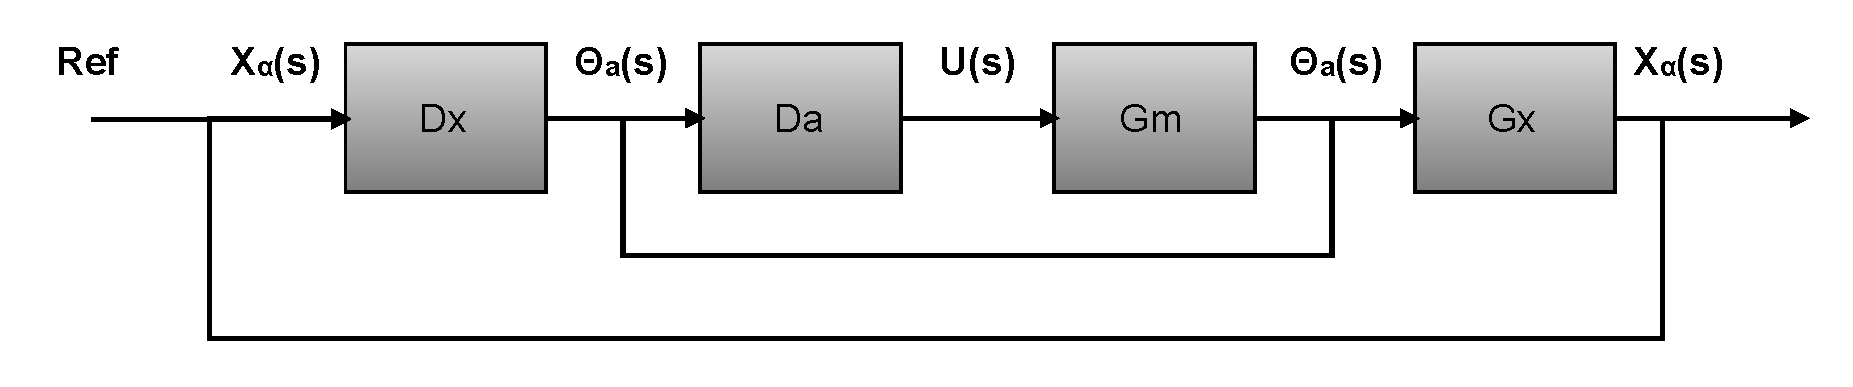
\includegraphics[width=\textwidth]{IPBlock}
\caption{Block diagram of the inverted pendulum system with inner and outer loop controllers.}
\label{fig:IPBlock}
\end{figure}

If the inner loop is faster than the outer loop then it can be assumed to be irrelevant when designing the outer loop controller.

\todo[inline,author=Jacob]{For the rest of this section: Use root locus to design Dx controller (Maybe parts of next section can be used here), then design Dm controller while keeping in mind it should be faster than Dx. I'd like for the angle of the stick to somehow be shown as a disturbance in the system and relate the redefinition to feedforward control for better disturbance rejection if possible. Tune parameters in the end as inner loop will have an effect on outer loop.}


\section{Controller with a 2nd right half plane pole added}
\todo[author=Jacob, inline]{A lot of this only applies for 2nd order system which this is not. I already wrote it without considering that so this section might have to be deleted but I'm leaving it for now.}
This controller adds a zero and a pole to the system and thus have three variables that needs to be chosen: The gain and the locations of the zero and the pole. The pole has to be located somewhere in the right half plane and the zero in the left. Their locations influence the root locus of the system.

To make the system as stable as possible a fast rise time and low overshoot is desirable. From the specifications the overshoot is set as maximum 10\% with no requirements for the rise time. The damping ratio, $\zeta$, can be found from the overshoot percentage, $M_p$, by \autoref{eq:IPOvershoot}.
\begin{subequations}
\begin{flalign}
& M_p=100\exp^{\frac{-\pi\zeta}{\sqrt{1-\zeta^2}}}<10\%  \\
& \zeta = \sqrt{\frac{\left(\ln{\frac{M_p}{100}}\right)^2}{\pi^2+\left(\ln{\frac{M_p}{100}}\right)^2}}  \\
& \zeta > \sqrt{\frac{\left(\ln{\frac{10\%}{100}}\right)^2}{\pi^2+\left(\ln{\frac{10\%}{100}}\right)^2}} = 0.59 \label{eq:IPOvershoot}
\end{flalign}
\end{subequations}

The damping ratio then has to be larger than 0.59 in order to have a overshoot of less than 10\% as specified. The rise time, $t_r$, is approximated by \autoref{eq:IPRisetime}.
\begin{flalign}\label{eq:IPRisetime}
& t_r =\frac{2.2}{\zeta\omega_n} 
\end{flalign}

In order to get as fast a rise time as possible the natural frequency and damping ratio both needs to be maximized. The natural frequency can be found on the root locus by the length from the poles to the origin. The damping ratio is found by the angle from the imaginary axis to the poles. As both $\zeta$ and $\omega_n$ are dependent on the pole locations it's possible that the fastest response time comes with a damping ratio below 0.59. The goal of this controller is to minimize \autoref{eq:IPRisetime} but maintaining a damping ratio above 0.59.

The location of the pole, and zero and the gain can thus be decided in order to achieve final pole locations with as far away from the origin as possible while having an angle to the imaginary axis that corresponds to $\zeta=0.59$.

%For the inverted pendulum it's also worth to consider a controller that keeps the arm at zero radians as well as it has a much harder time controlling the arm when out of the upright position. Therefore two controllers will be made: A single-input single-output (SISO) controller that only controls the angle of the stick and a single-input multiple-output (SIMO) controller that controls both the angle of the stick and the arm. 
%\todo[inline,author=Jacob]{If time allows. Otherwise just SISO.}

%\section{Single input single output controller for the inverted pendulum}
%For the SISO controller at least a zero or pole must be introduced along with the P-controller in the system in order to move the pole in the right half plane to the left half plane. For the pole in the right half plane to cross into the left half plane a pole must be added either in 0 to cancel the zero or in the right half plane forcing both off the real axis and allowing them to circumvent the zero in 0 and enter the stable region.

